\chapter{Środowisko uruchomieniowe aplikacji}
\thispagestyle{chapterBeginStyle}
Dedykowanym środowiskiem dla implementowanego systemu jest platforma Windows 10. Do prawidłowego funkcjonowania aplikacji, konieczna jest wcześniejsza instalacja kompilatora języka C++\footnote{Kompilator języka C++: \url{https://www.mingw-w64.org/downloads/}} oraz interpretera języka Python\footnote{Interpreter języka Python: \url{https://www.python.org/downloads/}}.\\

\begin{figure}[H]
	\centering
	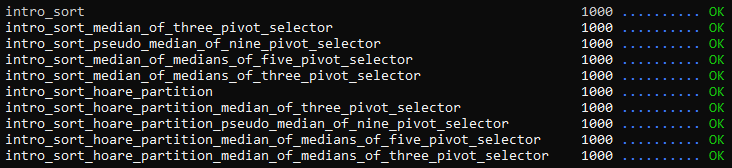
\includegraphics[width=0.9\textwidth]{img/screen}
	\caption[]{Fragment ekranu w trakcie działania silnika testującego}
	\label{fig:screen}
\end{figure}

% wykorzystanie biblioteki standardowej pythona oraz C++

\section{Zmienne środowiskowe}
Ponieważ parametry wejściowe powinny być współdzielone przez wszystkie składowe systemu, dane te są przekazywane za pomocą zmiennych środowiskowych. Każda ze zmiennych określa konkretną lokalizację na dysku systemowym:

\begin{itemize}
	\setlength\itemsep{0em}
	\item \MONOBOLD{CONFIG\FF DIRECTORY} - lokalizacja pliku konfiguracyjnego,
	\item \MONOBOLD{TEST\FF DIRECTORY} - lokalizacja pośrednich plików testowych,
	\item \MONOBOLD{PLOT\FF DIRECTORY} - lokalizacja wynikowego pliku wizualizacji.
\end{itemize}

\section{Biblioteki zewnętrzne}
W systemie wykorzystywano następujące biblioteki języka C++ w podanych wersjach:
\begin{itemize}
	\setlength\itemsep{0em}
	\item \MONOBOLD{fmt:7.1.3} - formatowane wyjście z interpolacją napisów,
	\item \MONOBOLD{nlohmann-json:3.9.1} - deserializacja pliku w formacie json,
	\item \MONOBOLD{scnlib:0.4} - parsowanie pliku w formacie csv.
\end{itemize}

Silnik graficzny wykorzystuje poniższe biblioteki języka Python:
\begin{itemize}
	\setlength\itemsep{0em}
	\item \MONOBOLD{scipy:1.7.1} - implementacje algorytmów numerycznych,
	\item \MONOBOLD{numpy:1.21.3} - agregacja danych liczbowych,
	\item \MONOBOLD{matplotlib:3.4.3} - tworzenie wizualizacji,
	\item \MONOBOLD{pandas:1.3.4} - parsowanie pliku w formacie csv,
	\item \MONOBOLD{SciencePlots:1.0.9} - naukowy styl wykresów.
\end{itemize}

\section{Cykl pracy programu}
Pracę ze środowiskiem można podzielić na trzy części. Na początku tworzony jest plik konfiguracyjny w formacie json.
Następnie, w oparciu o przygotowaną konfigurację, uruchamiany jest silnik testujący, który generuje pośrednie pliki wyjściowe. W ostatnim kroku uruchamiany jest silnik graficzny, który w oparciu o pliki wyjściowe pochodzące z silnika testującego, przygotowuje ostateczną wizualizację wyników. Ponieważ przy starcie silnika graficznego weryfikowana jest poprawność wszystkich plików pośrednich, każdy z kroków wykonywany jest sekwencyjnie, zaś cały program działa synchronicznie.\\

\section{Przykładowy plik konfiguracyjny}
Plik konfiguracyjny to dokument tekstowy w formacie json, zawierający wszystkie parametry potrzebne do przeprowadzanie testów.
W pliku ten można wyodrębnić dwie główne części. Część pierwsza zawiera parametry konfiguracyjne wspólne dla wszystkich testów, jak np. tytuł zestawu testowego, nazwa pliku wyjściowego czy rozmiar generowanej wizualizacji. W części drugiej zawarte są parametry unikatowe dla poszczególnych testów. Do parametrów tych należą m. in. opisy osi rzędnych i odciętych, generatory danych wejściowych dla poszczególnych testów oraz tytuły dla każdego wykresów. Dokładny spis wszystkich parametrów zawarty jest na końcu tego rozdziału. Poniżej znajduje się przykładowy plik konfiguracyjny.

\newpage
\lstinputlisting[language=json, caption=Przykładowy plik konfiguracyjny, captionpos=b]{chapters/pseudocodes/config-example.json}

\begin{table}[H]
	\centering
	\def\arraystretch{1.5}
	\begin{tabular}{ll}
		\multicolumn{2}{c}{}                									\\ \hline
		\BOLD{title}			& tytuł wizualizacji							\\ \hline
		\BOLD{output}			& nazwa pliku wyjściowego						\\ \hline
		\BOLD{prefix}			& prefiks dodawany do nazw plików pośrednich	\\ \hline
		\BOLD{grid}				& układ wykresów na wizualizacji $(x,y)$		\\ \hline
		\BOLD{size}				& rozmiar wizualizacji $(x,y)$					\\ \hline
		\BOLD{invariants}		& rozmiar tablicy oraz liczba powtórzeń			\\ \hline
		\BOLD{range}			& rozmiar tablicy								\\ \hline
		\BOLD{begin}			& początkowy rozmiar tablicy					\\ \hline
		\BOLD{end}				& końcowy rozmiar tablicy						\\ \hline
		\BOLD{step}				& inkrement podczas zmiany rozmiaru tablicy		\\ \hline
		\BOLD{repeats}			& liczba powtórzeń dla każdego z testów			\\ \hline
		\BOLD{plots}			& osobne konfiguracje dla poszczególnych wykresów \\ \hline
		\BOLD{type}				& rodzaj testu 									\\ \hline
		\BOLD{metadata}			& parametry graficzne dla pojedynczego wykresu 	\\ \hline
		\BOLD{title}			& tytuł wykresu 								\\ \hline
		\BOLD{xlabel}			& podpis osi odciętych 							\\ \hline
		\BOLD{ylabel}			& podpis osi rzędnych 							\\ \hline
		\BOLD{xcolumn}			& dane do osi odciętych 						\\ \hline
		\BOLD{ycolumn}			& dane do osi rzędnych 							\\ \hline
		\BOLD{xmin}				& minimalna wartość na osi odciętych 			\\ \hline
		\BOLD{xmax}				& maksymalna wartość na osi odciętych 			\\ \hline
		\BOLD{legend}			& pozycja legendy 								\\ \hline
		\BOLD{functions}		& funkcje pomocnicze drukowane na wykresie 		\\ \hline
		\BOLD{soirtings}		& wyniki testów drukowane na wykresie 			\\ \hline
		\BOLD{label}			& podpis linii 									\\ \hline
		\BOLD{color}			& kolor linii 									\\ \hline
		\BOLD{linestyle}		& styl linii 									\\ \hline
		\BOLD{expression}		& generator dla funkcji pomocniczej				\\ \hline
		\BOLD{algorithm}		& algorytm dla przeprowadzanego testu			\\ \hline
		\BOLD{generator}		& generator danych wejściowych przeprowadzanego testu \\ \hline
	\end{tabular}

	\caption[]{Opis parametrów zawartych w pliku konfiguracyjnym.}
	\label{tab:configuration}
\end{table}

